\section{Accessing records}

\begin{figure*}[t]
	\centering
	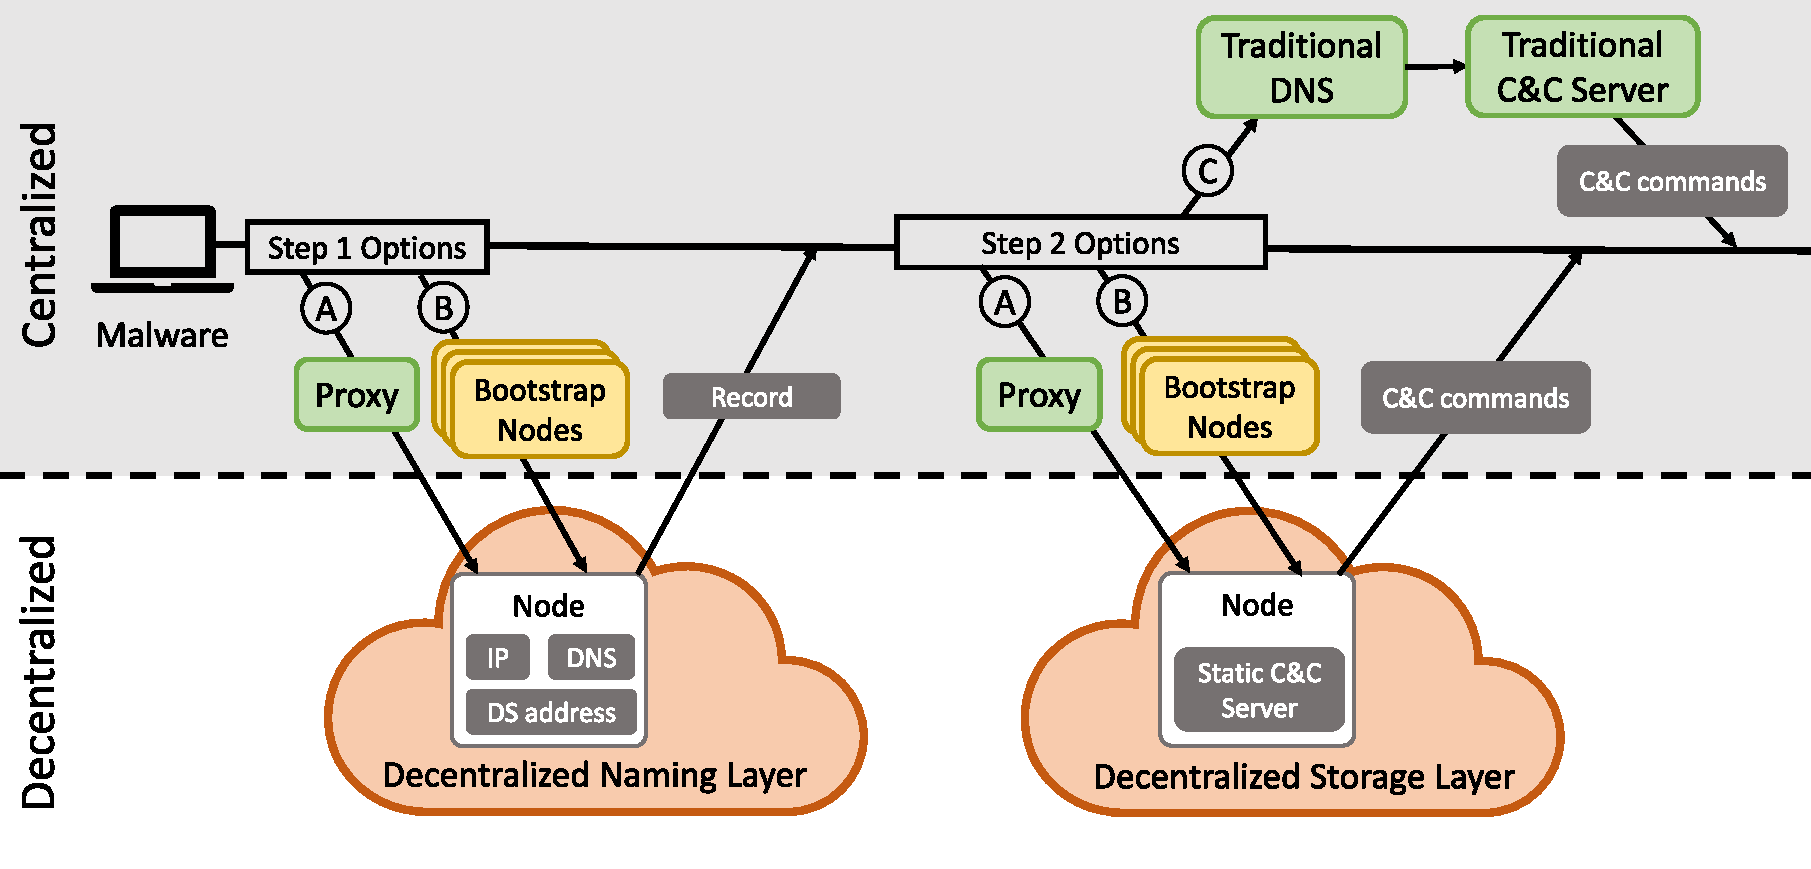
\includegraphics[width=\textwidth]{figs/malware_contacting_cnc.pdf}
	\caption{Malware must pass through centralized ``chokepoints'' to reach 
		decentralized systems, some of which might be good points for defender 
		interventions.}
	\label{fig:malware_contacting_cnc}
\end{figure*}

We have established that malware requires a naming layer to access its C2 
centers, and 
that blockchain-based naming systems are attractive options for implementing 
such a naming layer. 
We will now discuss the fundamental requirements of distributed naming systems 
and how 
these requirements present challenges and advantages to defenders. The first 
such fundamental 
requirement is accessing the distributed system.

To access name records stored on any distributed system like a blockchain, 
infected hosts must 
first obtain access to the blockchain itself. Accessing any distributed, 
peer-to-peer system for 
the first time requires learning the address of at least one participating 
node. In general, there 
are two methods for finding such an address: connecting to a 
proxy that already knows how to reach a member of the system, or acting 
as a full member of the system yourself and utilizing its peer-to-peer 
discovery protocol. The 
latter approach requires knowing a list of ``bootstrap nodes.'' For example, 
Ethereum uses a list 
of bootstrap nodes that are hard-coded into various client 
implementations. Bitcoin 
stores lists of nodes in DNS TXT records maintained by volunteers, as well 
as hard-coded 
lists~\cite{citation_needed}. A third option, a 
local discovery protocol that floods the network with 
messages looking for nodes, has not been adopted by any major 
blockchains that we are aware of. Such an approach would only be successful if 
the nodes running 
the blockchain were ubiquitous. It would also be very ``noisy'' and so 
unlikely to be favored by 
malware, so we do not discuss it further. 
Figure~\ref{fig:malware_contacting_cnc} shows the options 
infected hosts may choose from when connecting to a decentralized naming 
system, which we now 
discuss in more detail.

%Anything in Figure~\ref{fig:malware_contacting_cnc} in green is 
%centralized 
%enough to have to respond to a takedown request. Anything in yellow is 
%more difficult because taking it down would have collateral damage, and in 
%orange it's probably impossible to take down because it's truly 
%distributed and 
%very resilient to takedowns.



\subsection{Accessing blockchains using proxies}

To resolve a blockchain-based name to a website by using a proxy, users have 
several 
choices. Most large 
browsers, such as Safari, Chrome, and Firefox, do not support any 
blockchain 
naming systems natively. However, several extensions allow users to resolve 
names from ENS, 
Handshake, and Unstoppable Domains. These extensions rely on proxies that 
use 
DoH to send a resolution request to a server that can resolve the name. We 
note that such a server does not need to make a lookup to the chain every time 
it receives a request: it may cache names or keep track of its own database 
of names, which would simplify its implementation and speed up lookups 
significantly. 

Some browsers, such as Brave and Opera, claim to resolve certain naming 
systems 
natively. \randall{but when I tried this it didn't work? should try again 
	with 
	known websites and try Opera.} Both Brave and Opera rely on a proxy called 
Infura to resolve blockchain-based names. \randall{many citations 
	needed.} 

Some naming systems have partnerships with existing DNS resolvers. For 
example, 
NextDNS and Handshake have partnered to allow users who set their DNS resolver 
to NextDNS to resolve Handshake domains. Finally, some naming systems, 
such as 
Handshake, also provide stub resolver implementations that run locally on a 
user's computer. 

As a side note, the existence of competing naming systems in which name 
collisions are possible 
opens up the possibility of collision-based attacks. There is no governance 
system in place to prevent different systems from adopting the same TLDs and 
causing name collisions. In fact, several collisions already exist, both 
between blockchain-based systems themselves (Emercoin and Unstoppable both 
provide a ``.coin'' TLD) and between ICANN TLDs and blockchain-based systems 
(both Handshake and ICANN provide ``.music''). 
This means the record that a user receives when resolving a name with a 
collision depends on which resolution method they use. If the user has 
multiple 
proxies set up --- for example, multiple browser extensions installed that 
each 
try to resolve domains with a specific TLD --- then the record received will 
depend on which of those proxies takes precedence, which is not at all 
clearly 
defined. This lack of centralized governance enables several classes of 
attacks, such as squatting 
and phishing, which are beyond the scope of this paper.

Table~\ref{tab:proxies_and_tlds} provides a summary of the TLDs and 
proxies 
used by the blockchain naming systems we study. The list of proxies is not 
exhaustive, but 
represents 
a subset of the best-known proxies in use at the time of writing.
All of these proxies are 
centralized, which is good news for defenders: similarly to traditional 
registrars, they are vulnerable to legal takedowns. They can be served with 
legal takedown notices and compelled to stop giving access to abused domains, 
as long as they 
operate within a jurisdiction amenable to such efforts. A centralized proxy 
could also be taken 
down entirely by serving a takedown order to its hosting provider. While 
these interventions are 
not bulletproof, they are subject to the same advantages and disadvantages 
as 
interventions on traditional registrars. Thus, centralized proxies return 
the 
distributed naming ecosystem to a state similar to the DNS ecosystem, from a 
defender's point of view. 

\subsubsection{Case study --- BDNS takedown}
One example of an attempted proxy takedown is already known: 
the proxy known as ``Blockchain-DNS.info'' or BDNS. BDNS 
reported on their website that in April 2018, 
seven of their domain names were ``un-delegated'' and one of 
their API servers was shut down without 
warning~\cite{blockchain-dns-info-wayback}. The service then 
received a message from Spamhaus stating that several of 
BDNS's domains had been added to Spamhaus's blocklist. BDNS 
claimed that their browser extensions continued to resolve 
blockchain names using other endpoints, and directed users to 
a list of endpoints that were still 
working~\cite{github_bdns_wayback}. Finally, BDNS stated that 
they had moved some infrastructure to a friendlier hosting 
provider, PRQ, which states on its website that ``If 
[content] is legal in Sweden, we will host it, and will keep 
it up regardless of any pressure to take it 
down''~\cite{prq}. 

This takedown effort provides several lessons for defenders. 
First, it is possible to target a proxy when intervening with 
blockchain names. Defenders apparently tried two tactics: 
adding the proxy's endpoints to a widely used blocklist and 
taking down some domains and a hosting server entirely. 
The former tactic appeared to work well in locations where 
ISPs use Spamhaus's blocklist: BDNS stated that their 
proxy ``may be still unreachable in those parts of the 
world.'' However, the domain takedown was reportedly only 
partially effective. We conclude that care must be taken to 
enumerate all of the proxy's endpoints and shut them down 
simultaneously, since the proxy was reportedly still able to 
resolve blockchain names using the unaffected endpoints.  

At the time of writing, all of the endpoints listed in BDNS's 
Github repository~\cite{github_bdns_wayback} are either 
failing to resolve or failing to 
load a website, but it is unclear whether defenders performed 
a more successful 
takedown or the service shut down for other 
reasons. One endpoint, \texttt{bdns.io}, has 
apparently been sinkholed by ShadowServer, since its NS 
records now point to variants of the name 
sinkhole.shadowserver.org.\footnote{sinkhole-0[0-4].shadowserver.org
 and sinkhole-[a-b].shadowserver.org.}

We conclude that proxy takedowns are a viable method for 
defenders to intervene in the blockchain DNS ecosystem. 
However, while proxies simplify the process of 
connecting to a blockchain, they are not strictly necessary, 
which is bad news for defenders.

\subsection{The emergence of light clients}

When blockchains were first envisioned, most assumed that every participant in 
the network would be a ``full'' implementation of a node: it would contain 
enough state to reconstruct the entire history of the chain, all the way back 
to the first transaction. Additionally, each node would contribute to the 
blockchain by verifying every transaction it heard about. As various 
blockchains have grown over time, they have become too resource-intensive to 
run on anything other than a dedicated, powerful machine. Two 
resources serve as 
the constraints: first, CPU power, which is obviously necessary to perform 
mining but now is even a bottleneck for transaction verification on some 
machines, because so many transactions happen per 
second~\cite{citation_needed}. Second, disk 
space and speed. For example, Ethereum cannot be run on a machine with a hard 
disk drive anymore, because nothing slower than an SSD can keep up with the 
reads and writes required~\cite{citation_needed}. \randall{I 
	forget where I read this.} These resource constraints have 
given rise to the concept of a ``light client,'' a blockchain 
node with limited functionality that can fetch transactions 
from the chain but does not contribute by verifying 
transactions, mining, or broadcasting. Light clients are 
designed to run on laptops and mobile devices. As 
such, they are small enough to reasonably fit into a malware 
payload. 

Light clients enable malware to act as a first-class member 
of a blockchain, and discover other members of the chain 
using the chain's peer-to-peer discovery protocol without 
using a centralized proxy. Most peer-to-peer discovery 
protocols allow a client to connect to the blockchain for the 
first time by hard-coding a set of ``bootstrap nodes.'' In 
Ethereum, these bootstrap nodes are hard-coded into various 
implementations of the clients, and in Bitcoin, they are 
either hard-coded or accessible as TXT records stored at 
various trusted domains. The list of bootstrap nodes may also 
be configured by the user. If the 
malware chooses to use the bootstrap nodes that are 
hard-coded by default into the light client implementation, 
this may present a challenge for defenders, because taking 
down those bootstrap nodes may cause collateral damage to 
legitimate users attempting to join the chain. As such, 
bootstrap nodes are a more difficult place to stage an 
effective defender intervention than centralized proxies. 

Prohibiting malware from accessing a blockchain by intervening with the 
bootstrap nodes poses challenges compared to staging interventions at 
centralized proxies. If 
defenders take the bootstrap nodes down entirely, they risk causing 
collateral damage, by blocking 
access to the chain for licit users. However, because the IP addresses of 
the bootstrap nodes are 
public, defenders could also choose to add them to blocklists: IDSes, 
enterprise firewalls, or ISP 
routers can drop traffic intended for those destinations. The blocklist 
approach is very similar to 
blocking any other malicious IP addresses, and is subject to the usual 
challenges. Defenders must 
keep blocklists up-to-date as malware authors update the IPs they connect to, 
and malware authors 
could quickly pivot from using published IP addresses to IPs of nodes that they 
run 
themselves which are not publicly known. To the advantage of defenders, 
any time malware authors 
are forced to update the IP addresses that bootstrap nodes may be found at, 
they run 
afoul of the ``sunk cost'' problem where already-deployed malware that cannot 
be updated becomes 
useless. A similar argument applies if malware chooses to access bootstrap 
nodes using hard-coded 
DNS domain names instead of hard-coded IP addresses. Additionally, 
traditional interventions 
against domain names apply in that situation as well. Thus, while 
intervening at bootstrap nodes 
poses more of a challenge than intervening at centralized proxies, defenders 
still have viable 
options available.

\subsection{Naming record formats}

If malware successfully contacts the naming layer, it can then fetch the 
record that allows it to 
access its C2 center. 
This record can take several forms. The three that we observed in existing 
blockchain naming 
systems that might be useful to malware were IP addresses, 
traditional DNS domains, and addresses to distributed file storage 
systems like IPFS and SkyNet. We refer to these addresses as ``distributed 
storage'' (DS) 
addresses. Some naming systems allow users to store arbitrary text as 
records, which would allow 
malware to use nonstandard record types like links to social media posts. 

Each of these record types are subject to all of the traditional interventions 
that have already 
been described, except one: DS addresses. Distributed storage systems 
present a further challenge 
to defenders that goes beyond the challenges of decentralized naming. They 
enable malware authors 
to run an entire C2 center on a blockchain-based system that has no central 
authority capable of responding to a takedown request. In this respect, 
they provide a limited form 
of ``bulletproof'' hosting, and present their own unique challenges for 
both malware authors and defenders.

The decentralized storage systems available today do not offer the ability to 
host dynamic 
websites, so any C2 center implemented entirely on such a system must be a 
simple file with no 
dynamic content. Additionally, today's DS systems are 
content-addressed, which presents a challenge 
for malware authors that wish to hard-code the DS address of their C2 center 
into their payloads. 
If the file that represents the C2 server changes, its address will change as 
well, because the 
address is created from a hash of the file.

Some DS systems do not have redundancy, which raises the possibility of 
discovering the particular 
machine(s) responsible for hosting a C2 server and seizing it. 


\randall{where do I put this? Additionally, because all blockchain 
	records 
	are public, anyone can fetch those records including 
	defenders. You could theoretically scrape a blockchain looking for records 
	that match a known 
	malicious format or with malicious traits of some sort (owned by the same 
	wallet?) and try to seize 
	whatever those records point to.} 

Accessing a DS system is the same as accessing a distributed 
blockchain-based naming layer: you can do it either by proxy 
or by being a first-class member of the network, in which 
case you need bootstrap nodes. Theoretically, malware can go 
straight to the storage layer, but this is unlikely to be 
feasible given the way current DS systems are set up. The 
reason malware needs 
to use a naming layer to connect to the current generation of 
distributed file storage systems is because they're 
content-addressable. As soon as the file changes, so 
does its address, and the malware that knew the old address 
is useless. 
However, this is not a fundamental limitation of distributed 
storage systems --- a system could be designed in the future 
that doesn't have this limitation.

I don't know if IPFS/SkyNet have light nodes that could be 
part of a malware payload, but there does seem to be a trend 
in that direction as chains get heavier.